\documentclass{beamer}
\usepackage{beamerthemeshadow}
\usepackage{graphicx}
\usepackage{color}
\usepackage[utf8]{inputenc}
\usepackage{hyperref}
\usepackage[flushleft]{threeparttable}
\usepackage{lipsum}
\usepackage{caption}
\usepackage{tabularx}
\usepackage{url}
\usepackage[english,serbian]{babel}
\definecolor{royalblue}{RGB}{26, 22, 130}
\setbeamercolor{structure}{fg=royalblue}


\title{Tehničko i naučno pisanje}
\subtitle{-- Stiven Hoking --}
\author{ Ivana Milenković\\ \and Lazar Rajčić\\ \and Anđela Spasić\\ \and Nikola Stanojević }
\institute{Matematički fakultet\\Univerzitet u Beogradu}
\date{
	\footnotesize{Beograd, 2022.}	
}

\begin {document}
\begin{frame}
	\thispagestyle{empty}
	\titlepage
\end{frame}

\addtocounter{framenumber}{-1}

\begin{frame} \fontsize{9}{6}\selectfont
	\frametitle{Pregled}
	\tableofcontents[hidesubsections] 
\end{frame}
\section{Ko je Stiven Hoking?}

\begin{frame}[fragile]\frametitle{Ko je Stiven Hoking?}
	\begin{itemize} \fontsize{9}{6}\selectfont	
		\item  Stiven Hoking je bio engleski teoretski fizičar i kozmolog. Zbog njegovih doprinosa fizici smatran je za jednog od najvećih naučnika svog vremena. Njegovi doprinosi fizici se uglavnom nalaze u domenu našeg poznavanja crnih rupa. Zbog ovoga smatramo da je jako važno približiti njegova dostignuća ljudima.
\begin{figure}[h!]
  \centering
  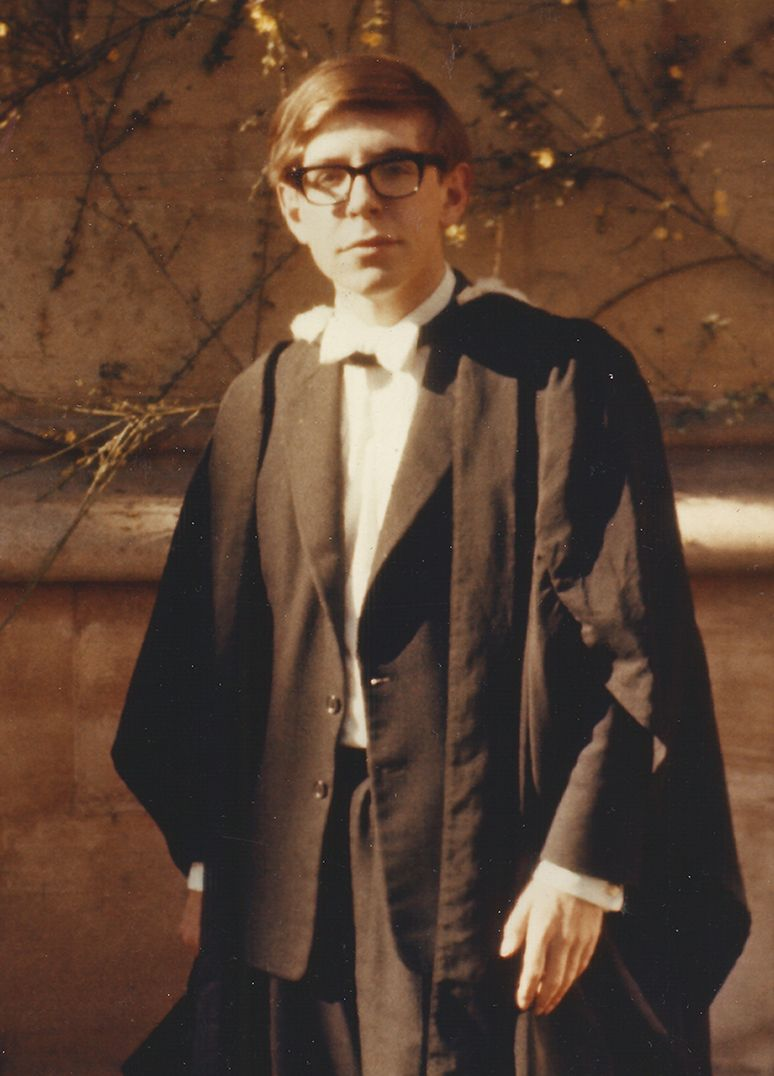
\includegraphics[width=0.3\textwidth]{Hoking,PreDijagnoze.jpg}
  \captionsetup{font=small}{Slika1: Hoking, na dodeli diploma 1960.}
  \label{fig:Hoking,PreDijagnoze}
  \end{figure}
	\end{itemize}
\end{frame}

\section{Život}
\begin{frame}[fragile]\frametitle{Rani život (Pre dijagnoze i dijagnoza)}
\begin{itemize}	 \fontsize{9}{6}\selectfont
		
\item  Hoking se rodio 8. Januara 1942. godine, tačno na tristotu godišnjicu smrti Galilea Galileja.
\item  U ranijim školskim godinama je dobio nadimak Ajnštajn.
\item  Zbog primedbi svog oca nastavio je da studira fiziku, a ne matematiku na Oksfordu. Osnovne studije je završio 1962. godine nakon čega prelazi na Kembridž univerzitet.
\end{itemize}
\end{frame}
